% ****** Start of file apssamp.tex ******
%
%   This file is part of the APS files in the REVTeX 4.2 distribution.
%   Version 4.2a of REVTeX, December 2014
%
%   Copyright (c) 2014 The American Physical Society.
%
%   See the REVTeX 4 README file for restrictions and more information.
%
% TeX'ing this file requires that you have AMS-LaTeX 2.0 installed
% as well as the rest of the prerequisites for REVTeX 4.2
%
% See the REVTeX 4 README file
% It also requires running BibTeX. The commands are as follows:
%
%  1)  latex apssamp.tex
%  2)  bibtex apssamp
%  3)  latex apssamp.tex
%  4)  latex apssamp.tex
%
\documentclass[%
 reprint,
%superscriptaddress,
%groupedaddress,
%unsortedaddress,
%runinaddress,
%frontmatterverbose, 
%preprint,
%preprintnumbers,
%nofootinbib,
%nobibnotes,
%bibnotes,
 amsmath,amssymb,
 aps,
%pra,
%prb,
%rmp,
%prstab,
%prstper,
%floatfix,
]{revtex4-2}

\usepackage[linesnumbered,ruled,vlined]{algorithm2e}
\let\oldnl\nl% Store \nl in \oldnl
\newcommand{\nonl}{\renewcommand{\nl}{\let\nl\oldnl}}% Remove line number for one line

%\usepackage{algorithm}
%\usepackage{algorithmic}
\usepackage{float}
\usepackage{subcaption}
\usepackage{graphicx}% Include figure files
\usepackage{dcolumn}% Align table columns on decimal point
\usepackage{bm}% bold math
\usepackage{hyperref}
\hypersetup{
    colorlinks=true,
    linkcolor=blue,
    citecolor=magenta
}
\captionsetup{justification   = raggedright,
              singlelinecheck = true}
%\usepackage{hyperref}% add hypertext capabilities
%\usepackage[mathlines]{lineno}% Enable numbering of text and display math
%\linenumbers\relax % Commence numbering lines

%\usepackage[showframe,%Uncomment any one of the following lines to test 
%%scale=0.7, marginratio={1:1, 2:3}, ignoreall,% default settings
%%text={7in,10in},centering,
%%margin=1.5in,
%%total={6.5in,8.75in}, top=1.2in, left=0.9in, includefoot,
%%height=10in,a5paper,hmargin={3cm,0.8in},
%]{geometry}
\bibliographystyle{apsrev4-1}

\begin{document}

\preprint{APS/123-QED}

\title{Qubit routing using Graph neural network aided Monte Carlo tree search}

\author{Animesh Sinha}
\email{animesh.sinha@research.iiit.ac.in}
\author{Utkarsh Azad}
\email{utkarsh.azad@research.iiit.ac.in}
\author{Harjinder Singh}
\email{laltu@iiit.ac.in}

\author{Jai Bardhan}
\author{Kalp Shah}
\author{Bhuvanesh Sridharan}
\affiliation{%
    Center for Computational Natural Science, International Institute of Information Technology, Hyderabad.
}%

\date{\today}% It is always \today, today,
%  but any date may be explicitly specified

\begin{abstract}
In near-term quantum hardware, the connectivity is limited to nearest neighboring qubits. This means that they support two-qubit operations only on the qubits that can interact with each other. To respect this constraint, compilers perform the task of qubit routing, i.e., to transforms quantum circuits either by including additional SWAP gates or by reversing existing CNOT gates to satisfy the connectivity constraints of the target topology. This article aims to provide an efficient solution for the qubit routing problem called QRoute, which minimizes the depth of these transformed circuits. We use the Monte Carlo tree search to perform qubit routing, which is aided by a Graph neural network that is used to evaluate the value function and action probabilities throughout the qubit routing procedure. Our procedure outperforms currently available qubit routing implementations on realistic circuit benchmarks while competing decently on random circuit benchmarks and is architecture agnostic.
\end{abstract}

\keywords{Qubit Routing, Quantum Compilation, Quantum Circuit Transformation, Reinforcement Learning, Monte Carlo Tree Search, Graph Neural Network}
\maketitle

%\tableofcontents

\section{\label{sec:intro}Introduction}

The present-day quantum computers, more generally known as Noisy Intermediate-Scale quantum (NISQ) devices \cite{preskill} come in a variety of hardware architectures \cite{IBMQ, GoogleSyncamore, RigettiAspen}, but there exists a few pervading problems across them. These problems constitute the poor quality of qubits, limited connectivity between qubits, and the absence of error-correction for noise-induced errors in the execution of gate operations. Hence, this places a considerable limitation on the number of quantum instructions that can be executed on them to perform some useful quantum computation. These instructions together can be realized as a sequential series of one or two-qubit gates acting on the qubits which can be visualized more easily as a quantum circuit as shown in Fig. \ref{fig:orig_circ}. 

To execute an arbitrarily given quantum circuit on the target quantum hardware, a compiler routine must transform it to satisfy the connectivity constraints of the topology of the hardware. These transformations usually include the addition of SWAP gates and the reversal of existing CNOT gates. Such transformation ensures that any non-local quantum operations are performed only between the qubits that nearest-neighbors and can interact with each other. This process of circuit transformation by a compiler routine for the target hardware is known as \textit{qubit routing}. The output instructions in the transformed quantum circuit would be following the connectivity constraints and would essentially result in the same overall unitary evolution as the original circuit \citep{qroute_dqn2}. 

In the context of NISQ hardware, this procedure is of extreme importance as the transformed circuit will, in general, have higher depth due to the addition of extra SWAP gates. This overhead in the circuit depth becomes prominent due to the high decoherence rates of the qubits and it becomes essential to find the most optimal and efficient strategy to minimize it. In this article, we present a procedure that we refer to as \textit{QRoute}. In this procedure, we propose to use the Monte Carlo tree search (MCTS) for the task of depth minimization, as an easier to train and better performing machine learning setting, which is aided by a Graph neural network (GNN) that is used to evaluate the value function and action probabilities throughout the compilation.

\textit{Structure}: In Section \ref{sec:qubit-routing}, we introduce the problem of qubit routing, the previous works that are done in the field, and show our work differs from them. Next, we represent the methodology of the QRoute algorithm in Section \ref{sec:method}. Then, in Section \ref{sec:results}, we benchmark the performance of our algorithm against other state-of-the-art quantum compilers. Finally, we discuss our results and  possible improvements in Section \ref{sec:discussion-conclusion}.

\begin{figure*}[t]
    \centering
    \begin{subfigure}[b]{0.30\linewidth}
        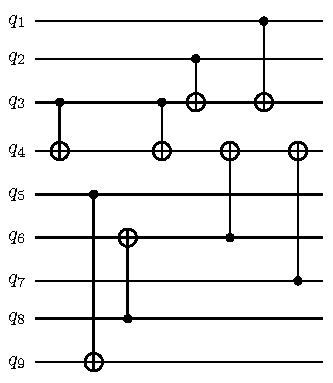
\includegraphics[width=\textwidth]{images/orig_circ.pdf}
        \caption{Quantum circuit\label{fig:orig_circ}}
    \end{subfigure}
    \begin{subfigure}[b]{0.30\linewidth}
        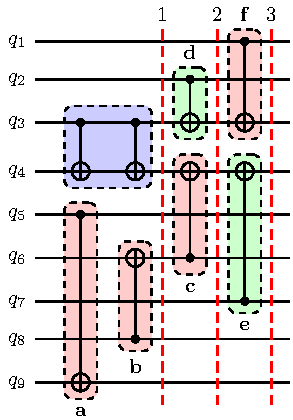
\includegraphics[width=0.85\textwidth]{images/sliced_circ.pdf}
        \caption{Decomposed circuit\label{fig:sliced_circ}}
    \end{subfigure}
    \begin{subfigure}[b]{0.33\linewidth}
        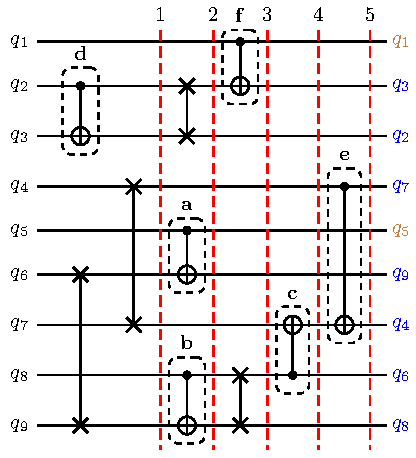
\includegraphics[width=\textwidth]{images/transformed_circ.pdf}
        \caption{Decomposed transformed circuit\label{fig:transformed_circ}}
    \end{subfigure}
    \caption{An example of qubit routing on a quantum circuit for 3$\times$3 grid architecture (Figure \ref{fig:3-3-arch}). (a) For simplicity, the original quantum circuit consists only of two-qubit gate operations. (b) Decomposition of the original quantum circuit into series of slices such that all the instructions present in a slice can be executed in parallel. Here, the two-qubit gate operations: $\{d,e\}$ (green) comply with the topology of the grid architecture whereas the operations: $\{a, b, c, f\}$ (red) does not comply with the topology (and therefore cannot be performed). Note that the successive two-qubit gate operations on $q_3\rightarrow q_4$ (blue) are redundant and are not considered while routing. (c) Decomposition of the transformed quantum circuit we get after qubit routing. Four additional SWAP gates are added that increased the circuit depth to $5$, i.e., an overhead circuit depth of $2$. Here, final qubit labels are represented at the end right side of the circuit. The qubits that are not moved (or swapped) are shown in brown ($\{q_1, q_5\}$), while the rest of them are shown in blue. Note that the overall unitary operation performed by the circuit is preserved despite the changes in the order of two-qubit gate operations}
    \label{fig:routing-example}
\end{figure*}

\begin{figure}[tp]
    \centering
    \begin{subfigure}[b]{0.42\linewidth}
        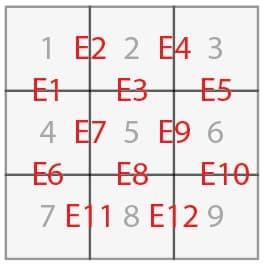
\includegraphics[width=\linewidth]{images/device-grid.jpg}
        \caption{3$\times$3 grid architecture\label{fig:3-3-arch}}
    \end{subfigure}
    \begin{subfigure}[b]{0.56\linewidth}
        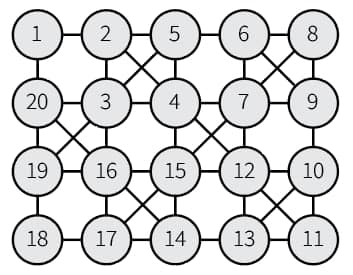
\includegraphics[width=\linewidth]{images/device-ibmqx.jpg}
        \caption{IBMQX-20 architecture}
    \end{subfigure}
    \caption{Examples of qubit connectivity graphs for some common quantum architectures}
    \label{fig:topology-example}
\end{figure}

\section{\label{sec:qubit-routing}Qubit Routing}
In this section, we begin by defining the problem of qubit routing formally and discussing the work done previously in the field.

\subsection{\label{sec:intro-defn}Describing the Problem}
The topology of quantum hardware can be visualized as a qubit connectivity graph (Fig. \ref{fig:topology-example}). Each node in this graph would correspond to a physical qubit which in turn might correspond to a logical qubit depending on whether they are being used in the execution of quantum instruction set or not. The quantum instruction set is also referred to as quantum circuit (Fig. \ref{fig:orig_circ}) is a sequential series of single-qubit and two-qubit gate operations that act on the logical qubits. Amongst these two type of gate operations, two-qubit qubit gates such as CNOT can only be performed between two logical qubits iff the there exist an edge between the nodes, i.e., the physical qubits, that corresponds to them respectively. This edge could be either be unidirectional or bidirectional, i.e., CNOT can be performed either in one direction or both directions. In this work, we consider only the bidirectional case, while noting that the direction of a CNOT gate can be reversed by sandwiching it between pair Hadamard gates acting on both control and target qubit \cite{}. 

Now, given a target hardware topology and a quantum circuit, the task of qubit routing refers to transforming this quantum circuit by adding series of SWAP gates such that all its gate operations then satisfy the connectivity constraints of the target topology (Fig. \ref{fig:transformed_circ}). Formally, for a routing algorithm $R$, we can represent this process as follows:
\begin{equation*}
\textrm{R}(circuit,\ topology) \rightarrow circuit'
\end{equation*}
Depth of \textit{circuit'} (transformed quantum circuit) will, in general, be more than that of the original circuit due to the insertion of additional SWAP gates. This comes from the definition of the term \textit{depth} in the context of quantum circuits. This can be understood by decomposing a quantum circuit into series of individual slices, each of which contains a group of gate operations that have no overlapping qubits, i.e., all the instructions present in a slice can be executed in parallel (Fig. \ref{fig:sliced_circ}). The depth of the circuit refers to the minimum number of such slices the circuit can be decomposed into, i.e., the minimum amount of parallel executions needed to execute the circuit. The goal is to minimize the overhead depth of the transformed circuit in w.r.t the original circuit.

We can breakdown this goal into solving two subsequent problems of (i) qubit allocation, which refers to the mapping of program qubits to logic qubits, and (ii) qubit movement, which refers to routing qubits between different locations such that interaction can be made possible \citep{}. In this work, we only focus on the latter problem of qubit movement and refer to it as qubit routing. However, we do note that qubit allocation is an important problem and can play important role in minimizing the effort needed to perform the latter.

\subsection{\label{sec:intro-related}Related Work}

The first major attraction for solving the qubit routing problem was the competition organized by IBM in 2018 to find the best routing algorithm. This competition was won by \citet{zulehner2018mapping}, for developing a Computer Aided Design-based (CAD) routing strategy. In subsequent years, this problem has been outlined and presented in many different ways. Some of them being graph-based architecture-agnostic solution by \citet{qroute_tket} and reinforcement learning in a combinatorial action space solution by \citet{qroute_dqn1}. In the latter, they also proposed the use of simulated annealing to search through the combinatorial action space, aided by a Feed-Forward neural network to judge the long-term expected compilation time. This was further extended to use Double Deep Q-learning and prioritized experience replay by \citet{qroute_dqn2}. 

Recently, Monte Carlo tree search, a popular reinforcement learning algorithm \citep{mcts_bandits_0, mcts_bandits_1, mcts_uct} previously proven successful in a variety of domains like playing puzzle games such as Chess and Go \citep{mcts_alphago} was used by \citet{qroute_mcts} to develop a qubit routing solution. However, they used MCTS in the context of minimizing the total volume of quantum circuits (i.e., the number of gates ignoring the parallelization). In our work, we focus on a formulation of MCTS given by \citet{mcts_assymetric}, that is adapted for better exploration of Asymmetric Trees. 

\begin{figure*}[t]
    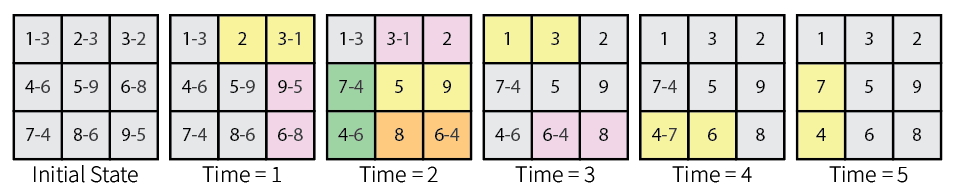
\includegraphics[width=\linewidth]{images/mcts_progress.png}
    \caption{\label{fig:routing-progress}Routing progress for 3$\times$3 grid architecture while for the quantum circuit in Fig. \ref{fig:orig_circ}. Initial state shows the gate scheduled on each qubit which gets executed as control and target qubit adjacent to each other via SWAPs. The final state (at time=$5$) shows t he final evolved qubit mapping. Here, each state (at time step=$t$) corresponds to the $t^{th}$ time slice in Fig. \ref{fig:transformed_circ}}
\end{figure*}

\subsection{\label{sec:intro-contribution}Our Contributions}

As mentioned before, in this work we propose to use the Monte Carlo tree search (MCTS), a reinforcement learning (RL) algorithm, for the task of total depth minimization. In the context of RL, we use an array of mutex locks to represent the information agent needs to know to make effective use of parallelization. Moreover, we propose a Graph neural network (GNN) that aids the MCTS in its exploration by evaluating function and action probabilities throughout the routing procedure. From these additional features, we aim to gain an agent that is not greedy immediately since it can only see the current state of the system and not effectively plan for the future. This also stabilizes the decision process which would have suffered from randomness if a method such as simulated annealing was used. Finally, we provide a simple python package that can be used to test and visualize routing algorithms with different neural net architectures, combining algorithms, reward structures, etc.

\section{\label{sec:method}Method}

The QRoute algorithm has four major segments:
\begin{enumerate}
    \item Maintaining and evolving an efficient representation of the current state of the entire system, which includes both the operations from the input circuit which are yet to be scheduled, and the current state of the solution.
    \item A value function and policy function approximator, here are graph neural network, which will evaluate the long term reward expected from the current state of the simulation.
    \item A Monte Carlo tree search agent, which will take the current state, and search over the set of actions available trying to find the optimal action based on immediate rewards and the long term evaluation offered by the value function approximator.
\end{enumerate}

In this section, we describe all these elements of our solution. \footnote{Code for the complete simulation and visualization is available on \protect\url{https://github.com/AnimeshSinha1309/quantum-rl}}

\subsection{\label{sec:method-state}State representation}

The QRoute algorithm takes an input circuit and makes progress through it iteratively, scheduling a list of parallelizable SWAP gates and CNOT gates subjected to the topology of the input hardware architecture. We refer to each such iteration as a timestep. At any given timestep $t$, the entire state of the compilation is captured by the state object $s_t$ at that timestep 
\begin{equation*}
    \textrm{s\textsubscript{t} = (circuit, device, s\textsubscript{t}.map, s\textsubscript{t}.progress, s\textsubscript{t}.locks)}
\end{equation*}

This is necessary and sufficient to capture the entire state of the system, in addition to this we also cache some alternate but useful representations of the state as listed in section \ref{sec:method-model}. We will describe the constituents of the state tuple in this subsection.

\subsubsection{\label{sec:method-state-circuit}Circuit Representation}

A circuit is a set of qubit $\mathbb{Q}$ together with an partially ordered set of operations on those qubits. 
\begin{equation*}
    O = \{(q_x, q_y) \mid q_x, q_y \in Q\}
\end{equation*}
The order in which two operations appear in the circuit is relevant to the overall unitary function implemented by it iff they share one or both of the qubits participating in them.

We convert the circuit to a lists of lists representation (as used by \citet{qroute_dqn2}), where for each logical qubit, $q_i$, we store the list of all other qubits that participate in two-qubit operations with $q_i$, in the order in which they appear in the logical circuit. 
This \textit{circuit} object is common over all the states in the simulation and does not evolve.

\subsubsection{\label{sec:method-state-device}Device Topology}

We need to have access to the topology of the target quantum devices to check whether a gate operation being performed in the input quantum circuit is feasible or not. This is stored as a graph in the \textit{device} object, all the nodes on the target hardware are nodes in the graph, and all pairs of adjacent qubits have an edge between them, as illustrated in figure \ref{fig:topology-example}.

We also maintain the shortest distances between all pairs of nodes, by running the Floyd-Warshall algorithm on the device graph, so that we can offer an intermediate reward function for bringing two qubits which participate in an operations that is waiting to be scheduled closer. 

\subsubsection{\label{sec:method-state-map}Node to Qubit Mapping}

Each node (or physical qubit) is mapped to either a logical qubit, or left empty. We maintain this mapping $Q \rightarrow N$, and evolve it using SWAP operations as shown in Fig. \ref{fig:routing-progress}. 
This mapping from the logical qubits to nodes is injective but not surjective.
The initial value of this mapping is either obtained through a qubit allocation algorithm, or assigned randomly.

\subsubsection{\label{sec:method-state-progress}Qubit Progress}

For each qubit, we maintain the progress it has made through the circuit. If $\textrm{s\textsubscript{t}.progress[q]} = k$, then the first $k$ operations in the logical circuit which $\textrm{q}$ participates in should have been scheduled in the output circuit before the current timestep $t$.

\label{para:method-state-circuit-gatecond}So a gate $(q_x, q_y)$ is waiting to be scheduled if and only progress of $q_x$ is $i$ and that for $q_y$ and $j$, and in the circuit object the (i+1)\textsuperscript{th} operation of $q_x$ is with $q_y$ and the (j+1)\textsuperscript{th} operation of $q_y$ is with $q_x$.


\subsubsection{\label{sec:method-state-mutex}Mutual Exclusion Locks}

Operations which are being scheduled must maintain mutual exclusivity with other operations over the nodes which participate in them. This is essential to minimizing the depth of the circuit since it models parallelizability of operations.

Since we can think of the nodes as ``resources" and the operations that are trying to use them as ``consumers", we note that our method is identical to the parallelization problems in classical computers, and we can adapt mutex locks \citet{mutex_dijkstra} to ensure mutual exclusion.

Different gates take different amounts of time to execute, for example if the primitive gates are CNOT on some hardware, then a SWAP gate will decompose to 3 CNOT gates and take 3 time-steps to complete execution. This is why we need to maintain the locks in the state object, since an operation from a previous timestep could still be holding locks on some nodes in the current timestep.

\begin{figure*}[t]
    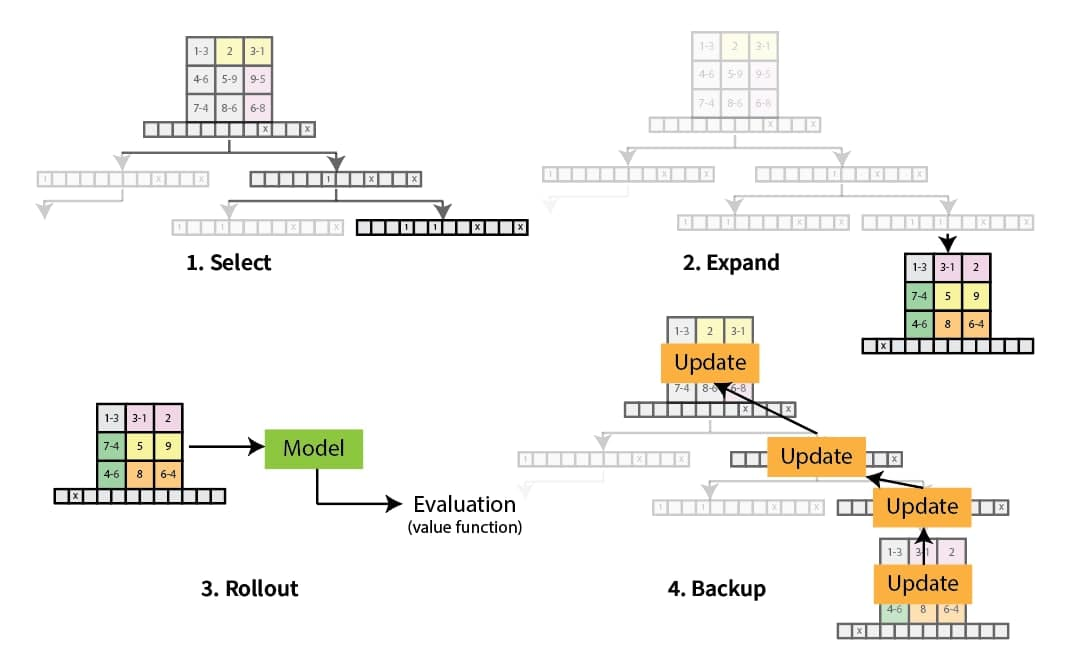
\includegraphics[width=\linewidth]{images/mcts-steps.jpg}
    \caption{\label{fig:mcts-explainer}
        Steps of Monte-Carlo tree search: (i) Select - Choose a mcts-state for exploration at current timestep, (ii) Expand - Calculating reward for newly encountered mcts-state and assign it as a child state, (iii) Rollout - Estimating long term value using a neural network for the state in the exploration tree, and (iv) Backup - Propagating value at leaf nodes upwards to update reward values of its ancestors.}
\end{figure*}

\subsection{\label{sec:method-mcts}Monte Carlo Tree Search}

Each timesteps starts off by greedily scheduling any CNOT gates that are waiting to be scheduled and are local on the hardware given the current qubit-to-node mapping. The CNOT gates, when scheduled, update the locks to ensure that the SWAP operations which will be generated for the same timestep can be executed in parallel with the CNOTs.
To find the optimal action, a parallelizable set of swaps for the state at any timestep, the QRoute algorithm employs a Monte Carlo tree search to search over the action space.

\subsubsection{\label{sec:method-mcts-state}In the Combinatorial Action Space}

There are exponentially many sets of SWAPs that together constitute an action. If there are $e$ edges on the target hardware, then we have $2^e$ possible actions, many of which break the mutual exclusivity constraint. We need to search the optimal action from the ones that don't. To search in this massive action space, we will build up our action one by one, starting off with an empty list, computing the set of SWAPs which do not violate the mutual exclusivity constraint, and choosing one of them, and iteratively continuing to build up our actions with more such gates. But since we may not always want to use the entirety of our swapping ability, we also add a ``commit'' action, which breaks out of this iterative process. The commit action is trivially chosen if there are no more SWAPs that are possible in the current timestep.

We represent this ``action'', as a boolean vector of length equal to the number of edges. This building up of actions shown in each individual rendering of the tree in figure \ref{fig:mcts-explainer}.

\subsubsection{\label{sec:method-mcts-state}The State of the Search}

The tree search needs to maintain an augmented form of the state, we shall call this mcts-state. This holds the state and a valid action from the state together with statistics on which state to go
\begin{itemize}
    \item A reference to the corresponding State
    \item A list of child mcts-states.
    \item N-values corresponding to each child mcts-state, number of iterations in which that child was explored.
    \item Q-values corresponding to each child mcts-state, mean estimated reward obtained when that child is explored.
    \item solution, a list of SWAPs that represents the action that corresponds to the mcts-state in search. 
\end{itemize}

Given an mcts-state $s$, the value function of that state is the expected total reward in the future.
\begin{equation}
    V(s) = \max_{s^\prime} Q(s, a)
\end{equation}
The Q-function is the total expected reward in the future after we took an action $a$ from state $s_t$.
\begin{equation}
    Q(s, a) = R(s, a, s^\prime) + \gamma V(s^\prime)
\end{equation}

\vspace\fill

\subsubsection{\label{sec:method-mcts-steps}How the Search Proceeds}

Monte Carlo Tree Search iteratively executes it's four phases of select, expand, rollout and backup.

\paragraph{} The first is a selection step which chooses the mcts-state we wish to explore in the current timestep. This choice is choosing the child mcts-state with the maximum Upper Confidence Bound on Trees (UCT) value for each mcts-state, and making our way down the tree till we reach a leaf node which has no explored children. UCT is the sum of the expected reward $Q$ and uncertainty in reward by a ratio $c$. This ratio trades off the exploration of the agent against the exploitation (choosing the best action based on current knowledge). 
\begin{equation}
    \textrm{UCT}(s, a) = Q(s, a) + c \frac{\sqrt{n(s)}}{n(s, a)} \times p(s, a)
\end{equation}
We recognize that running MCTS on this problem results in a highly assymetric tree, since some actions block a lot of other actions, and some actions don't interfere with any other action at all. So we add a Dirichlet noise term in the prior probabilities generated by our neural network to prevent our tree search from getting stuck down a single path. The formulation of MCTS for asymmetric trees is adapted from \citet{mcts_assymetric}

\paragraph{} The next step, Expansion, is triggered when we have taken an action from a mcts-state which has never been explored before. In this case, we create a new mcts-state, assign it to be the child state in our tree, and we compute the increase/decrease in reward due to that move and store it on the edge. The environment gives us a reward for bringing gates waiting to be scheduled closer together, actually scheduling gates, and finishing the entire compilation process. On the edge from the parent mcts-state to it's child, we assign a value equal to the increase in the expected reward from the parent to the child state. This value is 0 if the chosen action is commit.

\paragraph{} Once we are at a leaf node on the tree, we get our neural network to estimate the long term value of the state, in what is called the rollout stage. MCTS can also be performed without a neural network, in which case we randomly sample a bunch of paths to the leaf nodes and estimate the value of the current state based on the average reward received from those random runs. However, neural networks are much better at generalizing the features learnt from one state to another. This is particularly useful since very similar representations are encountered several times in the simulation.

\paragraph{} Finally, we have the evaluation of a node, and we need to update this information in it's parents. We take the value at the leaf nodes, and propagate it up the tree to it's ancestors, updating the q-values, which is the average expected reward from the parent, and the n-values, which is the number of times the particular action was taken.

\subsubsection{The final action choice}

Once the tree search is done, we use the tree to take our final action. We move down the tree again from the root, this time guided by the q-values and not by UCT, and move down till we find a commit action. We return the action, and move our root to the child state result from the commit action.

In addition, the n-values are representative of the probabilities with which each action was chose, and the q-value is the search enhanced estimate of the value function, we store both of these for the root node to train the policy and value function heads of our neural network.

\begin{algorithm}[t]
	\SetAlgoLined
	\DontPrintSemicolon
	\SetKwFor{Loop}{loop}{}{end loop}
	\KwData{state $s_t$} 
	\textbf{Initialize:} root $\leftarrow$ \textbf{new node}($s_t$, solution) \\
	\Loop{}{
	node $\gets$ root\\
	\Repeat{previous action was \textbf{expand}}{
		Compute \textbf{UCT} values using prior from model + noise \\
	action $\gets$ action from node with maximum UCT value \\
	\eIf{state.child[action] $\neq$ null}{
		node $\gets$ node.child[action]}{
		\eIf{action is commit}{
			next-state $\gets$ \textbf{step} (node.state, node.solution) \\
            %\sbox0{$\vcenter{\hbox{$\begin{array}{|c|c|c|c|c|} \hline 0 & 0 & 0 & \ldots & 0 \\ \hline\end{array}$}}$}
            $\hspace{0.13\textwidth}\vcenter{\hbox{$\begin{array}{|c|c|c|c|c|} \hline 0 & 0 & 0 & \ldots & 0 \\ \hline\end{array}$}}$\nonl \\
            next-solution $\leftarrow \underbrace{\vrule width0pt depth \dimexpr\dp0 + .3ex\relax\copy0}_{\textrm{\text{|device.edges|}}}$
			}
       		{next-state $\gets$ node.state \\
		 next-solution $\gets$ node.solution with a set bit at action index}%NestIF
	 state.child[action] $\gets$ \textbf{new node} (node.state, next-solution) \\
	\textbf{store} reward[node, action] $\gets$ \textbf{reward}(node.state, node.solution) - \textbf{reward}(next-state, next-solution) 
	}%MainIF
	}%Repeat
	final-state $\gets$ \textbf{step} (node.state, node.solution) \\
	reward $\gets$ \textbf{evaluation} from model of final-state
	\While{state $\neq$ root}{
		parent-action $\gets$ action which led to node from its parent node\\
		node $\gets$ node.parent \\
        reward $\gets$ reward[node, parent-action] + reward $\times$ discount-factor \\
        \textbf{update} node.q-value[action] with reward \\
        increment node.n-value[action] by 1	
	}%While
	}%Loop
	\textbf{memorize} the q-values and n-values at the root node for training the model later
\caption{Monte Carlo tree search}
\label{algmcts}
\end{algorithm}

\begin{figure*}[tp]
    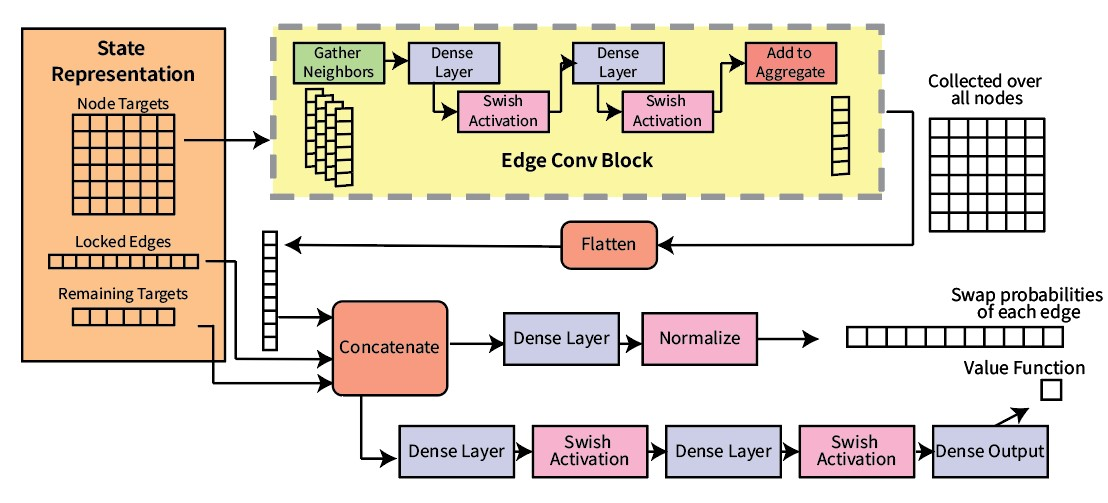
\includegraphics[width=\textwidth]{images/network-architecture.jpg}
    \caption{\label{fig:network-architecture}
        Graph Neural Network Architecture with a Value head and a Policy head}
\end{figure*}

\subsection{\label{sec:method-model}Neural Network Architecture}

Using the monte carlo tree search, we want to compute the q-values, which are the expected long term rewards, for each action from the current state. But these values are impossible to compute exactly, since it would involve visiting all leaf nodes in the subtree of the current state, and the number of these nodes grows exponentially with each new layer (timestep) in the tree. Therefore, it's necessary for us to stop after computing explicitly a few layers ahead in the future, and to heuristically evaluate the expected long term reward from the state.

Neural Nets are extremely good as function approximators. They are able to use the information gained from experiences from different runs, timesteps, and nodes. In this particular problem, very long term planning is not of particularly great use, optimally scheduling of the current and next few gates is more important. This leads us to feeding the following state representation to our neural network:
\begin{enumerate}
    \item Node Targets: If there are n nodes on the device, it's a matrix of $n \times n$ boolean values. Let the mapped to node i be $q_i$ and that to node j be $q_j$. The element at (i,j) is true if and only if ($q_i$, $q_j$) is a gate waiting to be scheduled. So each row at atmost one value that is true, but a column has one or more than one.
    \item Locked Edges: An equivalent representation of the locks in our state. It's a boolean vector of length equal to the number of edges, each element of the vector corresponds to an edge and is true if either of the nodes that the edge connects are locked (either from the previous state or due to the SWAPs we have already selected for the current action).
    \item Remaining targets: An integer vector of length equal to number of nodes. For each logical qubit, the number of operations that it will participate in which yet to be scheduled on the hardware.
\end{enumerate}

First, we need to get a feature vector for the gates which are currently waiting to be scheduled on the hardware, which is completely represented by the node targets matrix. This would be useful for both predicting the estimated value of the state as well as prior probabilities of which SWAP action should be chosen.

For each qubit, the SWAP operation it would ideally partake in depends primarily on it's target node, and on the SWAP operations that other nodes in it's neighborhood might be trying to partake in, competing for the same resources. It seems reasonable, therefore, that we can use a Graph Neural Network with the device topology graph for it's structure. Each node in the graph bears one row of the node-targets matrix. It is an assumption that the feature vector should only be dependent on some representation of the nodes and targets in it's local neighborhood on the device graph, but it's a reasonable one at that. And it promotes the use of message passing to convey this information about any node across it's neighborhood.

Formally, we take the node-targets vector and pass it through an edge convolution block \cite{nn_edge_conv} which uses two dense layers with swish activations \cite{nn_swish} and finally adds to aggregate all messages. These output feature vectors from the edge convolution block are collected over a bunch of nodes and flattened to form the total feature vector. The concatenation of this with the locked-edges vector and the remaining-targets vector will form the input to the value and policy heads.

The value head is 2 fully connected layers with Swish activations, and a final fully connected single neuron which has no activation.

The policy head is also just a single fully connected layer which has a output vector of size equal to the number of edges on device. We take the output of this layer, square it and then normalize it to convert the outputs of the neural network into a valid probability mass function. The outputs of this layer are interpreted as the probability of swapping the qubits which are on the ends of the corresponding edge.

\section{\label{sec:results}Results}
Here, we compare our algorithm QRoute against the other state-of-the-art algorirthms on various circuit benchmarks: Qiskit (and it's different variants) \citep{comp_qiskit}, Deep-Q-Networs (DQN) form \citep{qroute_dqn2}, Cirq \citep{comp_cirq} and CQC Pytket \citep{comp_pytket}.

\subsection{\label{sec:results-random}Random Test Circuits}

Our first benchmark is random circuits. These circuits are initialized with the same number of qubits as there are nodes on the device, and then two-qubit gates are randomly put between any pair of qubits, the number of such gates is varied from 30 to 150. We show the results of various frameworks in Fig. \ref{fig:results-random}.

\begin{figure}[t]
    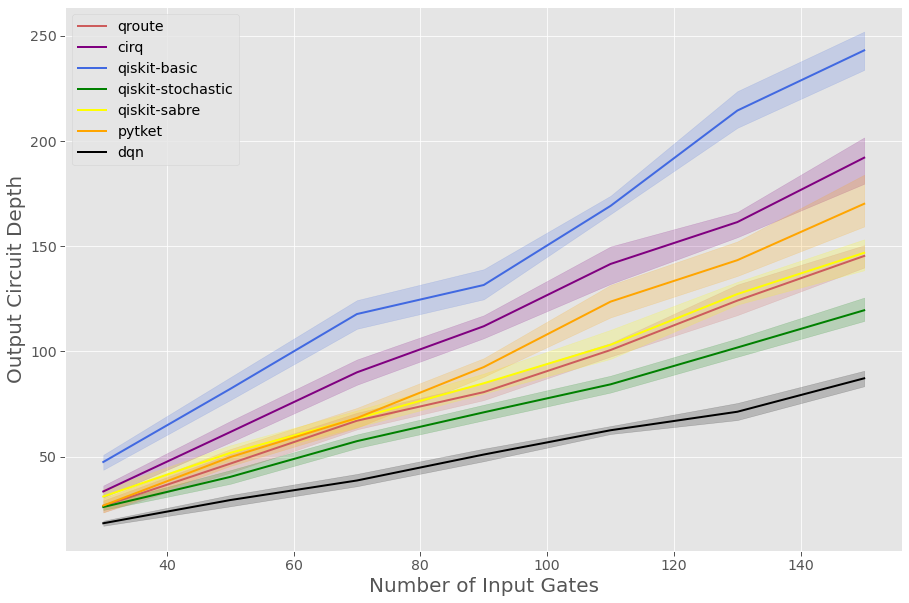
\includegraphics[width=\linewidth]{images/results-random.png}
    \caption{\label{fig:results-random}
        Comparative performance against other methods across real world hardware}
\end{figure}

In the frameworks compared, QRoute ranks third, performing worse than Qiskit Stochastic and Deep-Q-Networks. {\small (The results for the DQN were obtained from \citet{qroute_dqn2} and were not replicated.)}

Random circuits are a particularly difficult task for our method, since the neural network cannot generalize what it learnt on different random circuits in the training run to what will be useful for evaluation in the test run. Random circuits are also particularly difficult to train on. Nevertheless, our method is still competitive against all other frameworks and consistently performs better than most.

\subsection{\label{sec:results-small}Small Realistic Circuits}

Next we test on the set of all circuits which have 100 gates or less from the IBM-Q realistic quantum circuit dataset \cite{}. The comparative performance of all frameworks has been shown by plotting the depths of the output circuits summed over all the circuits in the test set. The plot is in figure \ref{fig:results-small}.

\begin{figure}[t]
    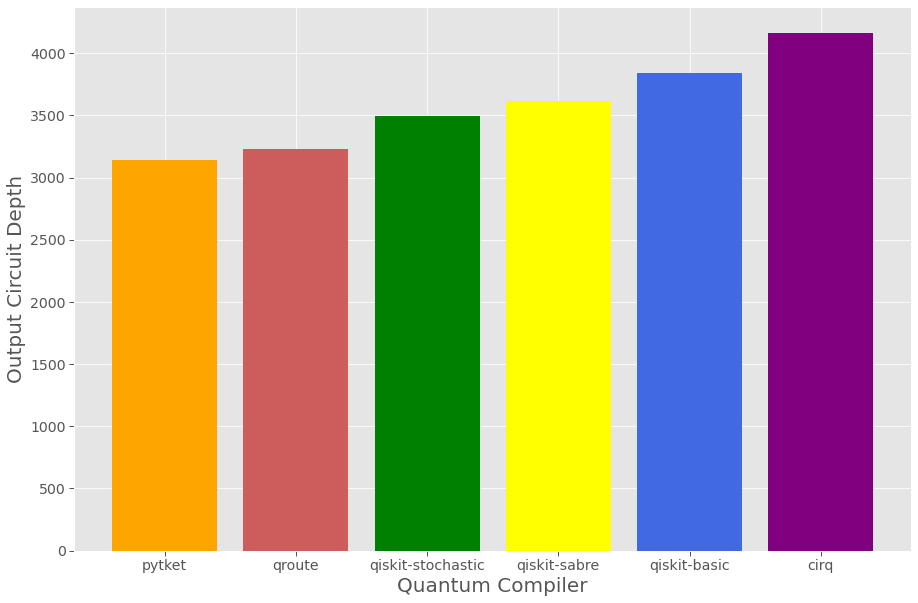
\includegraphics[width=\linewidth]{images/results-small.png}
    \caption{\label{fig:results-small}
        Scaling of Initial Depth overhead with size of hardware}
\end{figure}

Here, once again QRoute outperforms most of the other frameworks, but does slightly worse than CQC Pytket. We attribute some part of our worse performance to the lack of a qubit allocation algorithm, which is a relevant overhead on small circuits.

\subsection{\label{sec:results-realistic}Large Realistic Circuit}

For our final benchmark, we took 8 large circuits ranging from 154 gates to 5960 gates in its input from the IBM-Quantum realistic test dataset. We can clearly see that as the circuits get larger, our QRoute algorithm scales better than any other method and consistently produces the best results on almost all the test circuits. The results are detailed in table \ref{tab:large-circuits} and plotted in figure \ref{fig:results-large}.

The large circuits dataset was the largest dataset to train on and affords the QRoute the best opportunity to train on while being a harder task for all our compilers. Here the issue of qubit allocation is not a substantial part of the problem.

\begin{figure*}[t]
    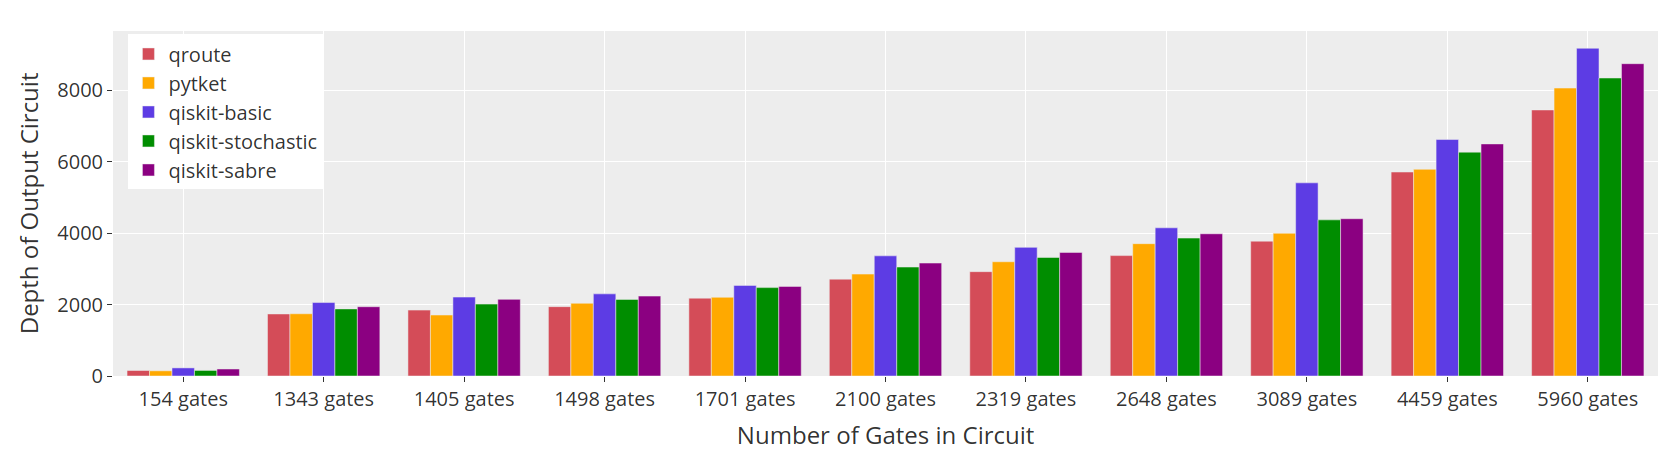
\includegraphics[width=\linewidth]{images/results-large.png}
    \caption{\label{fig:results-large}
        Performance on some large realistic test circuits}
\end{figure*}

\begin{table*}[t]
    \caption{\label{tab:large-circuits}%
        Results of our algorithm on a set of realistic test circuits
    }
    \begin{ruledtabular}
        \begin{tabular}{ll|rrrrr}
            \multicolumn{2}{c}{\textrm{Input Circuit}} & \multicolumn{5}{c}{\textrm{Output Circuit Depth}} \\
            
            \textrm{Name} & \textrm{Number of Gates} & \textrm{Qroute} & \textrm{PyTket Depth} & \textrm{Qiskit-Basic} & \textrm{Qiskit-Stochastic} & \textrm{Qiskit-Sabre} \\
            
            \colrule
            rd84\_142 	    &  154 &  154 &  145 &  227 &  156 &  196 \\
            adr4\_197 	    & 1343 & 1738 & 1743 & 2057 & 1879 & 1940 \\
            radd\_250 	    & 1405 & 1845 & 1707 & 2210 & 2013 & 2146 \\
            z4\_268 	    & 1498 & 1942 & 2036 & 2300 & 2145 & 2238 \\
            sym6\_145 	    & 1701 & 2180 & 2204 & 2537 & 2475 & 2509 \\
            misex1\_241 	& 2100 & 2712 & 2854 & 3365 & 3051 & 3163 \\
            rd73\_252 	    & 2319 & 2922 & 3199 & 3602 & 3320 & 3461 \\
            cycle10\_2\_110 & 2648 & 3372 & 3706 & 4150 & 3862 & 3983 \\
            square\_root\_7 & 3089 & 3776 & 3997 & 5409 & 4372 & 4404 \\
            sqn\_258 	    & 4459 & 5712 & 5788 & 6622 & 6269 & 6499 \\
            rd84\_253 	    & 5960 & 7450 & 8063 & 9178 & 8345 & 8746 \\
        \end{tabular}
    \end{ruledtabular}
\end{table*}

% Talk about time taken train the solution and to run it

\section{\label{sec:discussion-conclusion}Discussion and Future Scope}

This method of Quantum Circuit Transformation provides competitive and many a times superior performance to other methods. However, this is my no means a definitive solution to the task of Quantum Circuit Transformations, and offers great scope of improvement. We believe that the following are avenues in which the algorithm can be significantly improved:
\begin{itemize}
    \item Augmenting the Neural Network to take the future gates as an input. We propose to use a Transformer architecture for this, to learn a mapping from arbitrary-length list of gates to a feature vector which can be used in the Graph Neural Network to estimate the value function better.
    \item Finding more systematic approaches to manage the hyperparameters, e.g. Exploration-Exploitation tradeoff constant, Reward Parameters, etc.
\end{itemize}
Our software library allows easy access to implementing these neural networks by changing just a single file. We hope that this will aid future improvements and research in the task of quantum circuit transformations.

\appendix

\nocite{*}

\bibliography{qroute}% Produces the bibliography via BibTeX.

\end{document}
%
% ****** End of file apssamp.tex ******
